Dates (pour votre culture générale): Hahn (1879-1934), Banach (1892-1945).

Les théorèmes de Hahn-Banach sont des résultats d'analyse fonctionnelle
très importants. Ces théorèmes sont vus ici en deux formes:
les formes analytiques du théorème assurent qu'une forme linéaire
peut être étendue à tout l'espace en préservant certaines contraintes
iniatiales; les formes géométriques quant à elles sont des résultats
assurant qu'on peut séparer par des hyperplans deux convexes vérifiant
certaines hypothèses dans des espaces vectoriels normés.

\section{Formes analytiques}
\subsection{Espaces vectoriels sur $\mathbb{R}$}

\begin{thm}[Hahn-Banach -- Forme analytique (cas réel)] \label{hb:a1}
Soient $E$ un espace vectoriel sur $\mathbb{R}$, $G$ un sous-espace
vectoriel de $E$, $f: G \to \mathbb{R}$ une forme linéaire
et $p: E\to \mathbb{R}$ une application vérifiant les hypothèses suivantes:
\begin{itemize}
\item $\forall\lambda >0, \forall x \in E, p(\lambda x)=\lambda p(x)$
  (p est dite positivement homogène);
\item $\forall x,y \in E, p(x+y)\leq p(x)+p(y)$
  (p est dite sous-additive);
\item$\forall x\in G, f(x)\leq p(x)$.
\end{itemize}
Alors il existe $g:E\to\mathbb{R}$ forme linéaire étendant $f$ et telle
que $\forall x \in E, g(x)\leq p(x)$.
\end{thm}

\begin{proof}
  Supposons que $G\neq E$, sinon le résultat est immédiat.

  Supposons donc qu'il existe $x_0\in E\setminus G$. Montrons
  qu'il est possible d'étendre $f$ à $V = G\oplus \mathbb{R}x_0$
  comme annoncé dans le théorème.

  On doit montrer qu'il existe un réel $g(x_0)$ tel que pour
  tout $x = y+tx_0\in V$, $g(x)\leq p(x)$, c'est-à-dire
  $$f(y) + t g(x_0)\leq p(y + tx_0).$$

  Analysons les différents cas, selon le signe de $t$:

  \textbf{Cas 1, $t>0$}: la condition devient, par positive
  homogénéité de $p$ et linéarité de $f$
  $$\forall y\in G, g(x_0)\leq p\left(\frac{y}{t} + x_0\right)
  - f\left(\frac{y}{t}\right).$$
  Puisque $G$ est un sous-espace vectoriel, on peut réécrire la
  condition:
  $$\forall z\in G, g(x_0)\leq p(z + x_0) - f(z).$$

  \textbf{Cas 2, $t<0$}: la condition devient, par positive
  homogénéité de $p$ et linéarité de $f$
  $$\forall y\in G, g(x_0)\geq  f\left(\frac{-y}{t}\right)
  - p\left(\frac{-y}{t} - x_0\right).$$
  Puisque $G$ est un sous-espace vectoriel, on peut réécrire la
  condition:
  $$\forall w\in G, g(x_0)\geq f(w) - p(w - x_0).$$

  La question qu'on se posait revient donc à se demander s'il existe
  un réel satisfaisant les inégalités:
  $$\forall w, z\in G, f(w) - p(w - x_0)\leq g(x_0)\leq p(z + x_0) - f(z).$$

  Il suffit de montrer l'assertion:
  $$\forall w, z\in G, f(w) - p(w - x_0)\leq p(z + x_0) - f(z).$$

  Soient $z, w\in G$. On a $f(w + z)\leq p(w+z)$ par hypothèse
  sur $p$. Or puisque $$p(w + z)= p(w - x_0 + z +x_0)
  \leq p(w - x_0) + p(z + x_0)$$ par sous-additivité de $p$,
  et linéarité de $f$, on a l'inégalité.

  On peut donc poser, par exemple,
  $g(x_0)=\inf_{z\in G}p(z+x_0)-f(z)$.

  Pour finir la preuve, on utilise le lemme de Zorn, en considérant
  l'ensemble suivant, avec comme ordre l'inclusion (en considérant
  qu'une fonction $h_1$ prolonge une fonction $h_2$ \ssi{} le
  graphe de $h_1$ est inclus à celui de $h_2$):
  $$\mathcal{M}= \left\{(V, h)\mid  V\mbox{ sev. de $E$}, G\subseteq V,
    h: V\to\mathbb{R} \mbox{ linéaire, $h$ prolongement de $f$},
    h\leq p_{|V}\right\}.$$
\end{proof}

\subsection{Espaces vectoriels sur $\mathbb{C}$}

\begin{thm}[Hahn-Banach -- Forme analytique (cas complexe)]\label{hb:a2}
Soient $E$ un espace vectoriel sur $\mathbb{C}$, $G$ un sous-espace
vectoriel de $E$, $f: G \to \mathbb{C}$ une forme linéaire
et $p: E\to \left[0,+\infty\right[ $ une application vérifiant
les hypothèses suivantes:
\begin{itemize}
\item $\forall\lambda \in\mathbb{C},
  \forall x \in E, p(\lambda x)=|\lambda| p(x)$;
\item $\forall x,y \in E, p(x+y)\leq p(x)+p(y)$
  (p est dite sous-additive);
\item$\forall x\in G, |f(x)|\leq p(x)$.
\end{itemize}
Alors il existe $g:E\to\mathbb{C}$ forme linéaire étendant $f$ et telle
que $\forall x \in E, |g(x)|\leq p(x)$.
\end{thm}

\begin{proof}
  Remarquez que quel que soit l'élément $x\in G$ considéré,
  on a les égalités suivantes:
  \begin{IEEEeqnarray*}{rCl}
    i f(x) &=& - \Im(f)(x) + i\Re(f)(x);\\
    f(ix) &=& \Re(f)(ix) + i \Im(f)(ix).
  \end{IEEEeqnarray*}

  Par définition de l'égalité de deux nombres complexes
  (leurs parties réelles et imaginaires doivent être
  égales),
  on en déduit que $\Re(f)(ix) = -\Im(f)(x)$ et que
  $\Im(f)(ix) = \Re(f)(x)$. On peut donc exprimer $f$
  uniquement à l'aide de $\Re(f)$ de la manière suivante:
  $$f(x) = \Re(f)(x) - i \Re(f)(ix).$$

  L'application $\Re(f):G \to\mathbb{R}$ est une application
  $\mathbb{R}$-linéaire. Par le théorème de Hahn-Banach, cas
  réel, elle s'étend en une fonction $\mathbb{R}$-linéaire
  $h:E\to\mathbb{R}$.

  On pose $g$ l'application définie par
  $g(x)=h(x)- i h(ix)$ pour tout $x$ dans $E$.
  Donc $h$ correspond à la partie réelle de $g$.
  Il est aisé de vérifier qu'elle est $\mathbb{C}$-linéaire
  par calcul.

  Il reste à montrer que $g$ vérifie bien $|g|\leq p$.
  Soit $x\in E$. On a:
  \begin{IEEEeqnarray*}{rClr}
    |g(x)| & = & e^{-i\arg(g(x))} g(x) & \\
    & = & g(e^{-i\arg(g(x))}x) & \quad (\mbox{$g$ linéaire}) \\
    & = & \Re(g)(e^{-i\arg(g(x))}x) & \\
    & = & h(e^{-i\arg(g(x))}x) & \\
    & \leq & p(e^{-i\arg(g(x))}x) = p(x) & (\mbox{Thm. \ref{hb:a1}})
  \end{IEEEeqnarray*}

\end{proof}

\subsection{Espaces vectoriels normés}

\begin{thm}[Théorème de Hahn-Banach -- Forme analytique]\label{hb:a3}
  Soient $(E, \|.\|)$ un espace vectoriel normé sur $\mathbb{K}
  =\mathbb{R}$ ou $\mathbb{C}$, $G$ un sous-espace vectoriel
  de $E$ et $f: G\to\mathbb{K}$ linéaire continue.

  Alors il existe une fonction $g:E\to\mathbb{K}$ linéaire
  continue prolongeant $f$ telle que $\|f\| = \|g\|$.
\end{thm}

\begin{proof}
  On prend pour fonction $p: E\to\left[0, +\infty\right[$ la fonction
  $x\mapsto \|f\|\cdot\|x\|$. Elle vérifie toutes les hypothèses
  des théorèmes \ref{hb:a1} et \ref{hb:a2}.

  On peut donc prolonger $f$ en une forme linéaire $g$ telle que
  $|g(x)|\leq p(x)$ quel que soit $x\in E$. En particulier, cela
  implique que $g$ est continue car bornée sur la boule unité
  par la norme de $f$.

  Pour conclure il nous reste à montrer l'inégalité réciproque.
  Or pour tout $x\in G$ dans la boule unité, on a
  $|f(x)| = |g(x)|\leq \|g\|$, ce qui fournit l'inégalité
  désirée.
\end{proof}

\begin{rem}
  \textcolor{red}{
  Remarquez que le théorème n'exige \emph{pas} la complétude
  de l'espace vectoriel normé considéré.
}
\end{rem}


\subsection{Hahn-Banach et dualité}
Prouvons plusieurs corollaires des formes analytiques
du théorème de Hahn-Banach liés à la dualité.  Ils
constituent de petits exercices d'application des
théorèmes.

On considère un corps $\mathbb{K}$ qui est soit
celui des réels ou des complexes.

\begin{cor}\label{hb:a:cor1}
  Soient $(E, \|.\|)$ un espace vectoriel normé et
  $x_0\in E\setminus\{0\}$.

  Alors il existe $x^*\in E^*$, tel que $x^*(x_0)=1$
  et $\|x^*\|= \frac{1}{\|x_0\|}$.
\end{cor}

\begin{proof}
  Soit $G = \mathbb{K}x_0$. On considère l'application
  linéaire continue $f: G\to\mathbb{K}:tx_0\mapsto t$
  (la continuité est assurée car l'application est
  définie sur un espace de dimension 1).

  Calculons la norme de $f$:
  $$\|f\|=\sup_{\substack{t\in\mathbb{K}\\ \|tx_0\|\leq 1}}|f(tx_0)|=
  \sup_{\substack{t\in\mathbb{K}\\ |t|\leq\frac{1}{\|x_0\|}}}|t| =
  \frac{1}{\|x_0\|}.$$

  Pour conclure, il suffit d'utiliser le théorème \ref{hb:a3}.
\end{proof}

\begin{cor}\label{hb:a:cor2}
  Soient $(E, \|.\|)$ un espace vectoriel normé et
  $x_0\in E\setminus\{0\}$.

  Alors il existe $x^*\in E^*$, tel que $x^*(x_0)=\|x_0\|$
  et $\|x^*\|= 1$.
\end{cor}
\begin{proof}
  Soit $y^*$ fournie par le corollaire \ref{hb:a:cor1}.
  Il suffit de prendre $x^*= \|x_0\|y^*$.
\end{proof}

\begin{rem}\label{hb:a:norme}
  Soit $(E, \|.\|)$ un espace vectoriel normé. Soit $x\in E$.

  Quelle que soit la forme considérée $x^*\in E^*$, on a toujours
  que $|x^*(x)|\leq \|x^*\|\cdot \|x\|$.

  Par le corollaire \ref{hb:a:cor2}, on obtient l'égalité
  $$\|x\|=\max_{\substack{\|x^*\|\leq 1 \\ x^*\in E^*}}|x^*(x)|.$$
\end{rem}

\begin{cor}\label{hb:a:cor4}
  Soient $(E, \|.\|)$ un espace vectoriel normé, $F$
  un sous-espace vectoriel de $E$ qui n'est pas
  dense dans $E$ et $x_0\in (E\setminus\mathrm{adh}(F))$.

  Il existe $x^*\in E^*$ tel que $F\subseteq \mathrm{Ker}(x^*)$,
  $x^*(x_0)=1$ et $\|x^*\|=\frac{1}{d}$ où $d = d(x_0, F)$.
\end{cor}

\begin{proof}
  Soit $f: F\oplus \mathbb{K}x_0\to\mathbb{K}:y+tx_0\mapsto t$.
  Cette application est linéaire et on a $F\subseteq \mathrm{Ker}(f)$
  et $f(x_0)=1$.

  Rappelons que $d\neq 0$ car $x_0\notin \mathrm{adh}(F)$.

  Montrons que $f$ est continue.
  Soit $y + tx_0\in F\oplus \mathbb{K}x_0$ tel que
  $\|y + t x_0\|\leq 1$. On a, pour $t\neq 0$:
  $$\|y + tx_0\| = |t|\cdot
  \left\|x_0 - \left(-\frac{y}{t}\right)\right\|\geq d\cdot |t|.$$
  D'où $|f(y + t x_0)| = |t|\leq \frac{1}{d}$. Ceci montre que $f$
  est continue.

  En utilisant le théorème \ref{hb:a3}, on peut étendre $f$
  en une forme linéaire continue $x^*$ sur $E$ de même norme.
  Pour achever la preuve de l'assertion, il faut montrer l'inégalité
  $\|f\|\geq \frac{1}{d}$.

  Soit $\varepsilon >0$. Il existe $y\in F$ tel que
  $\|y-x_0\| - d <\varepsilon$ (définition d'infimum)
  c'est-à-dire $\| y - x_0\|\leq d + \varepsilon$.
  On a également l'inégalité
  $$\|f\|\geq \left|f\left(\frac{y - x_0}{\| y - x_0\|}\right)\right|
  =\frac{1}{\| y - x_0\|}
  \geq \frac{1}{d+\varepsilon}.$$
  On conclut en faisant tendre $\varepsilon$ vers 0.
\end{proof}

Pour conclure cette section, les deux exercices suivants sont laissés:
\begin{exo}\label{hb:a:exo1}
  Soit $(E, \|.\|)$ un espace vectoriel normé sur $\mathbb{K}$.
  Soit $F$ un sous-espace vectoriel de $E$. Montrer les équivalences
  suivantes:
  \begin{enumerate}
  \item ($x_0\in\mathrm{adh}(F)$) \ssi{} ($\forall x^*\in E^*,
    F\subseteq \mathrm{Ker}(x^*)\implies x^*(x_0) = 0$);
  \item ($\mathrm{adh}(F) = E$)  \ssi{}  ($\forall x^*\in E^*,
    F\subseteq \mathrm{Ker}(x^*)\implies x^* = 0$).
  \end{enumerate}
\end{exo}

Il existe une notation pour l'ensemble des formes linéaires
s'annulant sur un sous-espace vectoriel donné. Il est donc
possible de réécrire la question ci-dessus de manière plus
concise à l'aide de cette notation.

\begin{df}
  Soit $(E, \|.\|)$ un espace vectoriel normé sur $\mathbb{K}$.
  Soit $F$ un sous-espace vectoriel de $E$. On appelle
  annulateur de $F$ le sous-espace vectoriel suivant
  de $E^*$:
  $$F^\perp = \left\{x^*\in E^*\mid F\subseteq \mathrm{Ker}(x^*)\right\}.$$
\end{df}

\subsection{Bidualité}
Soit $(E, \|.\|)$ un espace vectoriel normé sur $\mathbb{K}$.
Il est possible de considérer les formes linéaires définies
sur le dual de $E$, étant donné qu'il s'agit d'un espace vectoriel
normé. On appelle cet espace le bidual de $E$, et
on le note $E^{**}$.

\begin{df}[Injection canonique]
  On appelle injection canonique l'application
  \begin{IEEEeqnarray*}{rCrCl}
    i & : & E & \to & E^{**} \\
    & & x & \mapsto & i(x).
  \end{IEEEeqnarray*}
  où pour tout $x\in E$, $i(x)$ est l'application définie par
   \begin{IEEEeqnarray*}{rCrCl}
      i(x) & : & E^* & \to & \mathbb{K} \\
      & & x^* & \mapsto & i(x)(x^*) = x^*(x).
    \end{IEEEeqnarray*}
\end{df}

Il est simple de vérifier que l'injection canonique est
bien définie (c'est-à-dire qu'elle est bien à image dans
$E^{**}$). De plus, l'injection canonique a les propriétés
suivantes:

\begin{prop}
  L'injection canonique est linéaire, continue et préserve
  la norme.
\end{prop}

\begin{proof}
  La linéarité est claire, car le dual est un espace
  d'applications linéaires, ce qui fournit le résultat.

  Quant à la préservation des normes, il suffit de constater
  les égalités suivantes (par le corollaire \ref{hb:a:cor2}):

  $$\|i(x)\|=\sup_{\substack{\|x^*\|\leq1\\ x^*\in E^*}}|x^*(x)|
  = \|x\|.$$
  Par cet argument, on a $\|i\| = 1$, ce qui implique
  que $i$ est continue.
\end{proof}

Les espaces qui s'identifient à leur bidual via l'injection
canonique sont dits réflexifs. Il existe des espaces qui sont
isomorphes à leur bidual, mais pas via l'injection canonique;
ces espaces sont appelés espaces de James.

\begin{prop}
  Si $E$ est réflexif, toute forme $x^*\in E^*$ atteint
  sa norme.
\end{prop}

\begin{proof}
  Soit $x^*\in E^*$. Il existe $x^{**}\in E^{**}$ de
  norme 1
  telle que $x^{**}(x^*)=\|x^*\|$, par le corollaire
  \ref{hb:a:cor2}. Par sujectivité de l'injection
  canonique, il existe $x\in E$ tel que $i(x)=x^{**}$.
  Il s'ensuit que $x^*$ atteint sa norme en $x$.
\end{proof}

\textbf{Remarque}: la réciproque est également vraie,
mais nous n'allons pas nous en préoccuper.

Dans le cas où l'espace n'est pas réflexif, il
existe donc des formes linéaires continues n'atteignant
pas leur norme. Donnons-en un:
\begin{ex}
  On considère $E = (c_0, \|.\|_\infty)$. Alors
  son dual $E^*$ s'identifie à $\ell^1$. Soit
  la suite $x = (\frac{1}{2^n})_{n\in \mathbb{N}}$
  qui est bien élément de $\ell^1$. Alors
  l'application suivante est bien élément de $(c_0)^*$:
  $$x^*:c_0\to\mathbb{K}:(y_n)_{n\in\mathbb{N}}\mapsto \sum_{n=0}^\infty x_ny_n.$$

  Montrons que $x^*$ n'atteint pas sa norme. Soit $y = (y_n)_{n\in\mathbb{N}}$
  un élément de la boule unité de $c_0$. Par définition, il existe
  $N$ un naturel tel que pour tout $n > N$, $|y_n|\leq \frac{1}{2}$. On a:
  $$|x^*(y)| \leq \sum_{n=0}^\infty \frac{|y_n|}{2^n} =
  \sum_{n=0}^{N} \frac{|y_n|}{2^n} + \sum_{n=N+1}^\infty \frac{|y_n|}{2^n}
  \leq \sum_{n=0}^{N} \frac{1}{2^n} + \sum_{n=N+1}^\infty \frac{1}{2^{n+1}}
  \leq 2 - \frac{1}{2^{N+1}}<2$$
\end{ex}

Montrons que tous les espaces de Hilbert sont réflexifs.
Pour ce faire, rappelons le théorème de représentation
de Riesz-Fréchet:
\begin{thm}[Théorème de représentation de Riesz-Fréchet]
  Soit $H$ un espace de Hilbert. Soit $x^*$ élément du dual de $H$.
  Il existe un unique élément $x\in H$ tel que pour tout $y\in H$,
  $x^*(y) = \langle y, x\rangle$.
\end{thm}

\textbf{Remarque}: Soit $H$ un espace de Hilbert.
L'application $H\to H^*: y \mapsto \langle$ $.$ $, y\rangle$ est
bijective (par le théorème de Riesz-Fréchet), une isométrie
et \emph{antilinéaire} (exercice).

Nous sommes maintenant armés pour montrer que tous les espaces
de Hilbert sont réflexifs.

\begin{thm}
  Tout espace de Hilbert $H$ est réflexif.
\end{thm}

\begin{proof}
  Munissons le bidual d'une structure d'espace de Hilbert.
  Pour ce faire, faisons d'abord de même pour le dual.

  Etant donné deux formes linéaires continues $u^*, v^*$ sur $H$,
  il existe $u, v$ deux éléments de $H$ leur correspondant (via
  le théorème de représentation de Riesz-Fréchet). On pose
  alors:
  $$\langle u^*, v^*\rangle = \langle v, u \rangle.$$

  Il s'agit bien d'un produit scalaire; les détails sont
  laissés à titre d'exercice (l'échange est important pour
  assurer la linéarité par rapport à la première composante).
  Ce produit scalaire engendre la même norme que la norme
  opérateur
  (puisque les représentants sont de même norme que
  les formes considérées). La complétude de $H^*$
  est assurée par la proposition \ref{lin:cpl:imp}.

  De la même manière, on munit le bidual de $H$ d'un
  produit scalaire, pour tous $u^{**}, v^{**}$ du bidual,
  soient $u^*, v^*$ leur représentants du dual, on pose:
    $$\langle u^{**}, v^{**}\rangle = \langle v^*, u^* \rangle.$$

  Soit $y^{**}\in H^{**}$. Montrons qu'il existe un élément
  de $y$ de $H$ tel que $y^{**}$ est l'image de $y$ par
  l'injection canonique.

  On considère $y$ le représentant de la forme linéaire continue
  $y^*$, elle-même représentante de $y^{**}$. Soient $x^*$ une forme
  linéaire continue et $x$ son représentant dans $H$. Alors:
  $$i(y)(x^*) = x^*(y) = \langle y, x\rangle$$
  et
  $$y^{**}(x^*) = \langle x^*, y^{*} \rangle = \langle y, x\rangle.$$

  Les deux correspondent ce qui  conclut la preuve.

\end{proof}

Vous pouvez consulter une autre preuve dans le document
\cite[p.~49]{refl:hilbert}.

\section{Formes géométriques}
\subsection{Hyperplans}
Soit $E$ un espace vectoriel sur $\mathbb{K}$
(le corps des réels ou des complexes).

\begin{df}
  Un sous-espace vectoriel $H$ de $E$ est dit hyperplan
  vectoriel s'il existe $e\in E$ non nul tel que
  $E = H\oplus \mathbb{K}e$.
\end{df}

Il existe une formulation équivalente en termes de formes linéaires:
\begin{prop}
  Soit $H$ un sous-espace vectoriel de $E$.
  Il s'agit d'un hyperplan vectoriel \ssi{} il existe une
  forme linéaire $f$ non identiquement nulle dont $H$ est
  le noyau.
\end{prop}

\begin{proof}
  Supposons que $H$ est un hyperplan vectoriel. Alors tout
  vecteur de $E$ s'écrit de manière unique sous la forme
  $x + te$ avec $t\in\mathbb{K}$ et $x\in H$.
  Il suffit de poser $f(x + te) = t$ pour avoir l'affirmation.

  Réciproquement supposons que $H$ est le noyau d'une application
  linéaire $f$ non nulle. Soit $e\in E$ un vecteur n'appartenant pas
  au noyau de $f$. Montrons que pour tout $x$ dans $E$, il existe
  $\lambda\in\mathbb{K}$ tel que $x-\lambda e\in H$;
  ceci impliquera $E = H + \mathbb{K}e$. Il suffit de prendre
  $\lambda = \frac{f(x)}{f(e)}$. On a bien $x-\lambda e\in H$.

  Il faut maintenant montrer l'unicité de cette écriture. Soient
  $a, b\in\mathbb{K}$, $u, v \in H$ tels que $x = u + ae = v+be$.
  En appliquant $f$, on obtient $af(e) = bf(e)$, d'où $a = b$
  et $u = v$.
\end{proof}

En plus des hyperplans vectoriels, on définit également les
hyperplans dits affines. Il s'agit de translatés d'hyperplans
vectoriels.
\begin{df}
  Un sous-ensemble $H$ de $E$ est dit hyperplan affine s'il
  existe $f$ une forme linéaire sur $E$ non nulle et un scalaire $\alpha$
  tels que $H = f^{-1}(\{\alpha\})$.
\end{df}

Supposons désormais que $(E, \|.\|)$ est un espace vectoriel
normé. On a le résultat suivant, qui lie continuité d'une
forme linéaire et si le noyau est fermé ou non.

\begin{prop}
  Soit $f: E \to\mathbb{K}$ une forme linéaire
  non identiquement nulle.

  Son noyau est fermé si et seulement si $f$ est continue.
\end{prop}

\textbf{Remarque}: l'application nulle est continue et son
noyau est fermé. Le cas est écarté de la proposition car
il est trivial.

\begin{proof}
  Si l'application est supposée continue, alors son noyau est
  fermé car il s'agit de l'image réciproque par $f$ du singleton
  $\{0\}$ qui est fermé.

  Réciproquement, supposons son noyau fermé. \'{E}tant donné que
  $f$ est non nulle, il existe $x_0$ dans le complémentaire du
  noyau, qui est ouvert (par hypothèse). On peut supposer $f(x_0)=1$
  (en normalisant le vecteur).

  Soit $r>0$ tel que $B(x_0, r)\subseteq E\setminus\mathrm{Ker}(f)$.
  On a donc $\forall z\in B(0, 1)$, $f(x_0 + rz )\neq 0$. Par
  linéarité de $f$, on obtient
  $\forall z\in B(0, 1)$, $f(z)\neq r^{-1}$.

  Pour conclure, il suffit de montrer que $|f(z)|< r^{-1}$ pour tout
  élément $z$ de la boule unité de $E$, une application linéaire
  étant continue si et seulement si elle est bornée sur la boule
  unité. Montrons que le
  cas complémentaire est impossible par l'absurde.

  S'il existe un élément $z$ de la boule unité de $E$ tel que
  $|f(z)|\geq r^{-1}$, alors il existe $y$ dans la boule unité
  tel que son image par $f$ est réelle positive et $f(y)\geq r^{-1}$
  (prendre $y = e^{-i\arg(f(z))}z$). En multipliant $y$ par une
  constante appropriée, on obtient un élément de la boule
  unité d'image $r^{-1}$ ce qui constitue une contradiction.

\end{proof}

\subsection{Introduction aux formes géométriques du
  théorème de Hahn-Banach}

Tout au long de cette section on considère un espace vectoriel
normé $(E, \|.\|)$ sur $\mathbb{R}$.

Le but de cette section est d'introduire les bases nécessaires
pour prouver les formes géométriques du théorème de Hahn-Banach.
Le théorème affirme qu'étant donnés deux convexes de $E$
vérifiant certaines hypothèses, il est
possible de les séparer ces derniers par un hyperplan, comme
illustré à la figure \ref{sep:ill}. Plus formellement:

% Figure pour illustrer la séparation au sens large de deux convexes
% par un hyperplan
\begin{figure}[!h]
  \begin{center}
    \caption{Séparation de deux convexes par des hyperplans dans $\mathbb{R}^2$}%
    \label{sep:ill}
    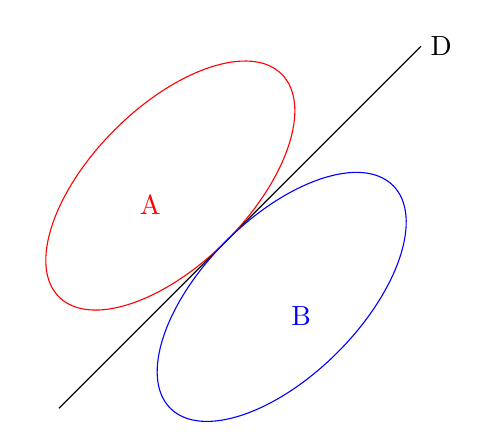
\begin{tikzpicture}
      \begin{scope}[rotate=315]
      \draw (1, -1) -- (1, 5.5) node[right] {D};
      \draw [red] (0 , 2) ellipse (1 cm and 2 cm) node[below left] {A};
      \draw [blue] (2 , 2) ellipse (1 cm and 2 cm) node[below right] {B};
    \end{scope}
    \end{tikzpicture}
\end{center}
\end{figure}

\begin{df}
  Soient $A$, $B$ deux sous-ensembles disjoints de $E$,
  $f:E\to\mathbb{R}$ une forme linéaire continue, $\alpha$ un
  réel et $H = f^{-1}(\{\alpha\})$ un hyperplan affine.

  $H$ sépare $A$ et $B$ au sens large si $\forall x\in A,
  f(x)\leq \alpha$ et $\forall x\in B, f(x)\geq \alpha$.

  $H$ sépare $A$ et $B$ au sens strict s'il existe
  $\varepsilon > 0$ tel que $\forall x\in A, f(x)\leq \alpha
  - \varepsilon$ et $\forall x\in B, f(x)\geq \alpha + \varepsilon$.
\end{df}

Pour parvenir à nos fins, on introduit une fonction appelée jauge
d'un convexe $C$:

\begin{df}
  Soit $C\subseteq E$ un convexe contenant 0 et ouvert.
  Pour tout $x$ dans $E$, on définit la jauge de $C$ en $x$ comme
  suit:
  $$j_C(x) = \inf\left\{\alpha > 0\mid x\in\alpha C\right\} =
  \inf\left\{\alpha > 0\mid \alpha^{-1}x\in C\right\}$$
\end{df}


Pour se familiariser avec cette fonction, vous êtes invité
à effectuer les exercices suivants:
\begin{exo}
  On considère le convexe $C = \left]\frac{-1}{2}, 2\right[$
  de $\mathbb{R}$.
  Effectuez les calculs suivants:
  \begin{IEEEeqnarray*}{rClCrCl}
    j_C\left(\frac{1}{2}\right) & = & \fbox{\phantom{AAAAAA}}
    &\qquad & j_C\left(-1\right) & = & \fbox{\phantom{AAAAAA}} \\
    j_C\left(\frac{-1}{2}\right) & = & \fbox{\phantom{AAAAAA}}
    &\qquad & j_C\left(2\right) & = & \fbox{\phantom{AAAAAA}} \\
  \end{IEEEeqnarray*}
\end{exo}

\begin{exo} \label{hb:g:j2}
  Soit $C$ un ouvert convexe de $E$ contenant $0$. Soit $x$ un élément
  de $E$. Montrer que quel que soit $\varepsilon > 0$,
  $$\frac{1}{j_C(x)+\varepsilon}x\in C.$$
\end{exo}

Pour prouver les formes géométriques du théorème de Hahn-Banach,
nous allons utiliser le résultat suivant.

\begin{prop}\label{hb:g:l}
Soient $C$ un ouvert convexe non vide de $E$ et $x_0\in E\setminus
 C$. Alors il existe un hyperplan fermé qui sépare $\{x_0\}$ et $C$
au sens large, c'est-à-dire:
$$\exists x^{*}\in E^*, \forall x \in C, x^*(x) < x^{*}(x_0).$$
\end{prop}

Prouvons plusieurs propriétés de la jauge d'un convexe qui serviront
dans la preuve de la proposition \ref{hb:g:l}.

\begin{lem} \label{lem:jc}
  Soit $C$ un ouvert convexe de $E$ contenant 0.
  \begin{enumerate}
  \item $\exists M> 0$, $\forall x\in E$, $0\leq j_C(x)\leq M\|x\|$.
    \label{lem:jc1}
  \item $C = \left\{ x\in E \mid j_C(x)<1\right\}$. \label{lem:jc2}
  \item La jauge d'un convexe est positivement homogène. \label{lem:jc3}
  \item L'application $j_C$ est sous-additive. \label{lem:jc4}
  \end{enumerate}
\end{lem}

\begin{proof}
  Montrons chaque point un à un.
  \begin{enumerate}
  \item Soit $r>0$ tel que $B(0, r)\subseteq C$. Posons
    $M = 2r^{-1}$. Soit $x\in E$ non nul. On vérifie facilement
    que $r\frac{x}{2\|x\|}\in B(0, r)\subseteq C$, d'où $x \in
    2r^{-1}\|x\|\cdot C$, ce qui donne le résultat.
  \item Soit $x\in C$. Soit $r> 0$ tel que $B(x, r)\subseteq C$.
    Alors il existe $\varepsilon >0$ tel que $(1+\varepsilon)x\in
    B(x, r)$. D'où $x\in \frac{1}{1+\varepsilon}\cdot C$ ce qui
    montre la première inclusion.

    Réciproquement, soit $x\in E$ tel que $j_C(x)<1$. Il existe
    donc $1 > \varepsilon > 0$ tel que $x\in \varepsilon \cdot C$.
    Par convexité de $C$, le segment joignant $0$ à
    $\frac{1}{\varepsilon}x$ est inclus à $C$; puisque
    ce dernier contient $x$, on a l'inclusion désirée.
  \item Soient $x$ un élément de $E$ et $\alpha$ un réel strictement
    positif. Pour tout $\beta > 0$, $\alpha x\in \beta\cdot C$, \ssi{}
    $x\in \alpha^{-1}\beta C$. D'où $j_C(\alpha x) = \alpha j_C(x)$ en
    passant à l'infimum sur $\beta$.
  \item Soient $x$, $y$  deux éléments de $E$. Soit
    $\varepsilon>0$. On a:%\in\left]0, 1 \right[$. Alors
    $\frac{1}{j_C(x)+\varepsilon}x\in C$ et
    $\frac{1}{j_C(y)+\varepsilon}y\in C$ (cf. exercice résolu \ref{hb:g:j2}).
    Par convexité de $C$, on a pour tout $t\in [0, 1]$:
    $$t\frac{1}{j_C(x)+\varepsilon}x +
    (1-t)\frac{1}{j_C(y)+\varepsilon}y\in C.$$
    En prenant $\displaystyle{t = \frac{j_C(x)+\varepsilon}
      {j_C(x) +j_C(y)+2\varepsilon}}$, on obtient
    $$\frac{x+y}{j_C(x) +j_C(y)+2\varepsilon}\in C. $$

    Par le point \ref{lem:jc2} et la positive homogénéité de la jauge d'un convexe,
    on obtient $j(x + y) < j_C(x)+j_C(y)+2\varepsilon$. On conclut
    en prenant $\varepsilon \to 0$.
  \end{enumerate}
\end{proof}

Nous pouvons donc procéder à la preuve de la proposition \ref{hb:g:l}
en utilisant ces propriétés.

\begin{proof}
Sans perte de généralité, on peut supposer $0\in C$; si ce n'est pas le cas,
on considère $y_0\in C$ et \og on translate \fg, c'est-à-dire on prouve la
propriété pour le convexe $C' = C - y_0$ et le point $x_0' = x_0 - y_0$ et on utilise
la linéarité de la forme obtenue pour avoir le résultat.

On pose $G = \mathbb{R}x_0$ et on considère la forme linéaire définie sur $G$
par $\forall t\in \mathbb{R}$, $f(tx_0) = t$. Alors pour tout $t$ réel, on a
$f(tx_0)\leq j_C(tx_0)$; si $t$ est négatif, c'est clair, et si $t$ est positif,
cela revient à montrer (puisque $j_C$ est positivement homogène)
que $1\leq j_C(x_0)$, ce qui est vrai car $x_0\notin C$.

Par la forme analytique du théorème de Hahn-Banach (théorème \ref{hb:a1}),
$f$ se prolonge en une forme linéaire $g$ sur $E$ vérifiant $\forall x \in E$,
$g(x)\leq j_C(x)$.
De plus, comme il existe une constante $M >0$ telle que tout élément
$x$ de $E$ vérifie $j_C(x) \leq M\|x\|$, la continuité de $g$ est assurée
sur $E$.

On considère l'hyperplan $H = g^{-1}(\{1\})$. Montrons qu'il sépare bien $C$ et
le singleton $x_0$. C'est immédiat car $g(x_0) = 1$ et tout élément $y$ de $C$
est tel que $g(y)\leq j_C(y) < 1$.
\end{proof}

Le corollaire suivant est laissé au lecteur à titre d'exercice. Vous êtes
invités à le montrer de plusieurs manières; en utilisant la proposition
précédente ou un des corollaires des formes analytiques.

\begin{exo}
  Montrer que $E^*$ sépare les points de $E$, c'est-à-dire si $x$, $y$
  sont des éléments de $E$, il existe $x^*$ une forme linéaire continue
  sur $E$ telle que $x^*(x)\neq x^*(y)$.
\end{exo}

En particulier deux éléments de $E$ sont égaux \ssi{} leur image
par toute forme linéaire continue coïncide.

\subsection{Théorème de Hahn-Banach: Formes géométriques}
Tout au long de cette section, on considère un espace vectoriel normé
$(E, \|.\|)$ sur $\mathbb{R}$.
\begin{thm}[Théorème de Hahn-Banach -- Première forme géométrique] \label{hb:g1}
  Soient $A$ un ouvert convexe non vide de $E$, $B$ un convexe non vide
  de $E$ tels que $A$ et $B$ sont disjoints. Alors il existe un hyperplan
  fermé qui sépare $A$ et $B$ au sens large.
\end{thm}

\begin{proof}
  Soit $C = A - B $. Il s'agit d'un convexe ouvert de $E$. La convexité
  se vérifie par calcul et pour montrer que $C$ est ouvert,
  il suffit de remarquer qu'il s'agit d'une union d'ouverts:

  $$ C = \bigcup_{b\in B} A - b =
  \bigcup_{b\in B} \left\{a - b \mid a\in A\right\}.$$

  \'{E}tant donné que $A$ et $B$ sont disjoints, $0\notin C$.
  Par la proposition \ref{hb:g:l}, il existe une forme linéaire
  continue $x^*$ telle que tout élément $x$ de $C$ a une image
  strictement négative. Il s'ensuit que pour tout élément $a$ de
  $A$, pour tout élément $b$ de $B$, $x^*(a - b) < 0$.

  Puisque $B$ est non vide, $\alpha = \sup_{x\in A}x^*(a)$ est fini. L'hyperplan
  $(x^*)^{-1}(\alpha)$ sépare $A$ et $B$ au sens large, ce qui conclut la preuve.
\end{proof}

Il existe une seconde forme géométrique du théorème de Hahn-Banach.

\begin{thm}[Théorème de Hahn-Banach -- Deuxième forme géométrique] \label{hb:g2}
  Soient $A$ un compact convexe non vide de $E$, $B$ un fermé convexe non vide
  de $E$ tels que $A$ et $B$ sont disjoints. Alors il existe un hyperplan
  fermé qui sépare $A$ et $B$ au sens strict.
\end{thm}

Introduisons un lemme utile dans la preuve du théorème

\begin{lem}\label{hb:g:l2}
  Soit $(F, \|.\|)$ un espace vectoriel normé sur $\mathbb{K}$ (où
  $\mathbb{K}= \mathbb{R}$ ou $\mathbb{C}$), $A$, $B$ deux convexes
  non vides disjoints de $F$, $A$ compact et $B$ fermé.

  Alors il existe $\varepsilon > 0$ tel que $A_\varepsilon =
  A + B(0, \varepsilon)$  et $B_\varepsilon = B
  + B(0, \varepsilon)$ sont disjoints.
\end{lem}
\begin{proof}
  Supposons par l'absurde que cela soit faux. Pour tout naturel $n$ non
  nul, il existe $x_n\in A_{1/n}\cap B_{1/n}$. Alors $x_n$ s'écrit comme
  $a_n + z_n$ pour certains $a_n\in A$, $z_n\in B(0, 1/n)$ et comme
  $b_n + w_n$ pour certains $b_n\in B$, $w_n\in B(0, 1/n)$.

  Par compacité séquentielle de $A$, il existe une sous-suite de
  $(a_n)_{n\in\mathbb{N}}$, notons-la $(a_{n_k})_{k\in\mathbb{N}}$, un élément
  $a$ dans $A$ tel que   $(a_{n_k})_{k\in\mathbb{N}}$ converge
  vers $a$. Puisque les suites $(z_n)_{n\in\mathbb{N}}$ et
  $(w_n)_{n\in\mathbb{N}}$ convergent vers $0$, on déduit que
  la sous-suite  $(b_{n_k})_{k\in\mathbb{N}}$ de
  $(b_{n})_{n\in\mathbb{N}}$ converge vers $a$, ce qui implique $a$
  dans $B$ (car $B$ est fermé), ce qui contredit $A$ et $B$ disjoints.
\end{proof}

Prouvons la seconde forme géométrique du théorème de Hahn-Banach à l'aide
du lemme ci-dessus.

\begin{proof}
  Soit $\varepsilon> 0 $ tel que $A_\varepsilon$ et $B_\epsilon$ (au sens du
  lemme \ref{hb:g:l2}) sont disjoints. Puisque ce sont des ensembles ouverts,
  convexes, non vides et disjoints, il existe $x^*$ forme linéaire continue,
  $\alpha$ un nombre réel tel que pour tout $a\in A_\varepsilon$,
  $x^*(a)\leq\alpha$ pour tout $b\in B_\varepsilon$, $x^*(b)\geq \alpha$.
  (par la première forme géométrique).

  On a pour tout $a$ dans $A$, $x^*(a)\leq \alpha - \varepsilon\|x^*\|$ et
  de manière analogue,
  pour tout $b$ dans $B$, $x^*(b)\geq \alpha +\varepsilon \|x^*\|$, ce qui
  conclut la preuve.

\end{proof}

\subsection{Généralisation aux espaces vectoriels complexes}
Soit $(E, \|.\|)$ un espace vectoriel normé sur $\mathbb{C}$. Il est
possible de généraliser les formes géométriques du théorème de Hahn-Banach
aux espaces vectoriels sur le corps des complexes.


Voici une première généralisation de la première forme géométrique.
\begin{thm}[Hahn-Banach -- Première forme géométrique, cas complexe]\label{hb:g:c1}
  Soient $A$ un ouvert convexe non vide de $E$, $B$ un
  convexe non vide de $E$ tels que $A$ et $B$ sont disjoints. Il existe
  $x^*$ une forme linéaire non nulle sur $E$ et $\alpha$ un nombre réel tels que:
  $$A\subseteq \left\{x\in E\mid \Re(x^*)(x) \leq \alpha\right\} \mbox{ et }
  B\subseteq \left\{x\in E\mid \Re(x^*)(x) \geq \alpha\right\}.$$
\end{thm}

\begin{proof}
  Par la première forme géométrique (dans le cas réel), il existe une forme continue $f$
  $\mathbb{R}$-linéaire sur $E$ telle que
  $$A\subseteq \left\{x\in E\mid f(x) \leq \alpha\right\} \mbox{ et }
  B\subseteq \left\{x\in E\mid f(x) \geq \alpha\right\}. $$

  On conclut en posant $x^*(x) = f(x) - if(ix)$ pour tous $x$ dans $E$.
  La linéarité est à vérifier à titre d'exercice et
  elle est bien continue car: $$|x^*(x)|\leq |f(x)|+|f(ix)|\leq
  \|f\|\|x\|+\|f\|\|ix\| = 2 \|f\|\|x\|.$$
\end{proof}

Il est possible d'avoir un résultat similaire en considérant
des modules plutôt que les parties réelles de la forme linéaire,
au coût d'une hypothèse supplémentaire sur un des ensembles.
Introduisons d'abord une définition.

\begin{df}
  Soit $A$ un sous-ensemble de $E$. $A$ est dit équilibré
  (ou $\mathbb{C}$-symétrique) si quel que soit
  l'élément $v$ de $A$ et le complexe $\lambda$ de module 1 considérés, le vecteur
  $\lambda{}v$ est un élément de $A$.
\end{df}

Le résultat est le suivant:

\begin{cor}\label{hb:g:cc1}
  Soient $A$ un ouvert convexe non vide \emph{équilibré} de $E$, $B$ un
  convexe non vide de $E$ tels que $A$ et $B$ sont disjoints. Il existe
  $x^*$ une forme linéaire non nulle sur $E$ et $\alpha$ un nombre réel tels que:
  $$A\subseteq \left\{x\in E\mid |x^*(x)| \leq \alpha\right\} \mbox{ et }
  B\subseteq \left\{x\in E\mid |x^*(x)| \geq \alpha\right\}. $$
\end{cor}


\begin{proof}

  Par le théorème \ref{hb:g:c1}, il existe $x^*$ linéaire continue telle que
  $$A\subseteq \left\{x\in E\mid \Re(x^*)(x) \leq \alpha\right\} \mbox{ et }
  B\subseteq \left\{x\in E\mid \Re(x^*)(x) \geq \alpha\right\}. $$

  Alors pour tous $b$ dans $B$,
  on a: $|x^*(b)|\geq \Re(x^*)(b) \geq \alpha$.
  Soit $a\in A$. On a (par linéarité de $x^*$ et par $\mathbb{C}$-symétrie
  de $A$):
  $$|x^*(a)| = x^*(e^{-i\arg(x^*(a))}a) =
  \Re(x^*)(e^{-i\arg(x^*(a))}a)\leq \alpha.$$
\end{proof}

Adaptons la seconde forme géométrique du théorème de Hahn-Banach.
\begin{thm}[Hahn-Banach -- Deuxième forme géométrique, cas complexe]
  Soient $A$ un compact convexe non vide de $E$, $B$ un fermé
  convexe non vide de $E$ tels que $A$ et $B$ sont disjoints. Il existe
  $x^*$ une forme linéaire non nulle sur $E$, $\alpha$ un nombre réel et
  $\varepsilon > 0$ tels que:
  $$A\subseteq \left\{x\in E\mid \Re(x^*)(x) \leq \alpha-\varepsilon\right\}
  \mbox{ et }
  B\subseteq \left\{x\in E\mid \Re(x^*)(x) \geq \alpha+\varepsilon\right\}. $$
\end{thm}

\begin{proof}
  Par le lemme \ref{hb:g:l2}, il existe $\varepsilon > 0$ tel que $A_\varepsilon$
  et $B_\varepsilon$ (en reprenant les notations du lemme) sont disjoints.

  Alors par le théorème \ref{hb:g:c1}, il existe une forme linéaire continue $x^*$,
  un réel $\alpha$ tel que:
  $$A_\varepsilon\subseteq \left\{x\in E\mid \Re(x^*)(x) \leq \alpha\right\} \mbox{ et }
  B_\varepsilon \subseteq \left\{x\in E\mid \Re(x^*)(x) \geq \alpha\right\}. $$

  Alors pour tout $a$ dans $A$, pour tout $z$ dans $B(0, \varepsilon)$,
  $\Re(x^*)(a + z) \leq \alpha$.

  Soit $a\in A$. Par linéarité de $x^*$, la dernière affirmation implique
  que pour tout $z$ dans la boule unité,
  $\Re(x^*)(a) + \varepsilon\Re(x^*)(z) \leq \alpha$.
  Puisque l'affirmation est vraie
  pour tous $z$ dans la boule unité, on peut
  passer au suprémum sur les $z$ et on obtient l'inégalité $\Re(x^*)(a)+
  \varepsilon \|x^*\|\leq \alpha$.
  Avec un calcul similaire, on peut conclure pour $B$.
\end{proof}

\textbf{Remarque}: il est possible d'écrire une version du résultat
utilisant des modules plutôt que des parties réelles dans les inégalités
à la manière du corollaire \ref{hb:g:cc1}. Vous êtes invités à écrire
le résultat et à le montrer à titre d'exercice.

\subsection{Applications}
Nous considérons à nouveau dans cette section un espace vectoriel
normé $(E, \|.\|)$ sur le corps des nombres réels. Nous allons
présenter plusieurs corollaires des théorèmes de Hahn-Banach.

Commencer par présenter une preuve alternative du corollaire \ref{hb:a:cor4},
qui utilise la forme géométrique du théorème de Hahn-Banach.
\begin{cor}
  Soit $F$ un sous-espace vectoriel de $E$ tel que $F$ n'est
  pas dense dans $E$. Alors il existe une forme linéaire non nulle
  continue s'annulant sur $F$.
\end{cor}
\begin{proof}
  Un sous-espace vectoriel est un convexe. Soit $x_0\in E\setminus\mathrm{adh}(F)$.
  Alors $\{x_0\}$ est un compact convexe de $E$ et $\mathrm{adh}(F)$
  est un sous-espace vectoriel (donc convexe) fermé ne contenant pas $x_0$.
  Par la deuxième forme géométrique de Hahn-Banach, il existe une forme
  linéaire $x^*$, un réel $\alpha$ et $\varepsilon >0$
  tels que $x^*(x_0)\geq \alpha + \varepsilon$  et
  pour tout $y\in F$, $x^*(y)\leq \alpha-\varepsilon$. En particulier, $x^*$ est majorée
  sur $F$ par une constante; il est facile de vérifier que $x^*$ s'annule
  sur $F$. On en déduit $\alpha \geq 0$ ce qui nous permet de conclure
  que $x^*(x_0)$ est non nul.
\end{proof}

\textbf{Remarque}: ce résultat a déjà été énoncé (cf. corollaire
\ref{hb:a:cor4}). Il est répété ici pour donner une preuve différente
qui utilise les formes géométriques de Hahn-Banach.

De manière similaire à l'annulateur d'un sous-espace vectoriel, on peut
définir un sous-espace vectoriel similaire du dual.
\begin{df}
  Soit $N$ un sous-espace vectoriel de $E^*$. On définit $N_\perp$
  comme le sous-ensemble de $E$ défini par:
  $$N_\perp = \left\{ x\in E\mid \forall x^*\in N, x^*(x) = 0\right\}$$
\end{df}

Il s'agit d'un sous-espace vectoriel fermé de $E$ : cela se peut montrer
en écrivant l'ensemble comme l'intersection des noyaux des éléments de $N$
qui sont fermés.

\begin{prop}
  Soit $F$ un sous-espace vectoriel de $E$. Montrer l'égalité
  $(F^\perp)_\perp = \mathrm{adh}(F)$.
\end{prop}

\begin{proof}
  On a clairement l'inclusion $F \subseteq (F^\perp)_\perp$, ce qui
  fournit $\mathrm{adh}(F) \subseteq (F^\perp)_\perp$.

  L'inclusion réciproque est fournie par le résultat de l'exercice
  \ref{hb:a:exo1} (la solution de l'exercice est donnée en annexe).
\end{proof}

Maintenant nous avons tous les outils nécessaires pour démontrer la
réciproque de la proposition \ref{lin:cpl:imp}.
\begin{thm}\label{lin:cpl:equ}
  Soient $(F, \|.\|_F)$, $(G, \|.\|_G)$ deux espaces vectoriels normés sur
  sur $\mathbb{K}$ ($\mathbb{R}$ ou $\mathbb{C}$).

  $\mathscr{L}(F, G)$ est un espace de Banach \ssi{} $G$ est un espace
  de Banach.
\end{thm}

\begin{proof}
  Il reste à prouver une implication. Supposons $\mathscr{L}(F, G)$ complet.
  Soit $(y_n)_{n\in\mathbb{N}}$ une suite de Cauchy dans $G$.

  Fixons un élément $x_0$ de la sphère unité de $F$, c'est-à-dire
  $\|x_0\|_F = 1$. Par le corollaire \ref{hb:a:cor2}, il existe
  donc un élément $x^*$ du dual de $F$ de norme 1 et tel que $x^*(x_0) = 1$.

  Pour tout naturel $n$, on définit l'application $f_n: F\to G$
  par $f_n(x) = x^*(x)y_n$ quel que soit $x$ dans $F$;
  il s'agit bien d'une application linéaire
  et continue. Montrons que la suite $(f_n)_{n\in\mathbb{N}}$ est une suite
  de Cauchy. Soient $n$, $m$ deux naturels, on a:
  $$\|f_n-f_m\| =
  \sup_{\substack{x\in F\\\|x\|_F = 1}}\|x^*(x)y_n - x^*(x)y_m\|_G =
  \|y_n - y_m\|_G \sup_{\substack{x\in F\\\|x\|_F = 1}} |x^*(x)| =
  \|y_n - y_m\|_G $$

  Puisque la suite $(y_n)_{n\in\mathbb{N}}$ est de Cauchy, il est immédiat
  par l'égalité précédente que la suite $(f_n)_{n\in\mathbb{N}}$ l'est
  également. Elle converge donc vers une application linéaire et continue
  $f$.

  La convergence au sens de la norme opérateur impliquant la
  convergence ponctuelle, on a donc
  $y_n = f_n(x_0)\xrightarrow[n\to+\infty]{} f(x_0)$, donc
  la suite $(y_n)_{n\in\mathbb{N}}$ est convergente.

\end{proof}

\begin{prop}\label{ker:sub:mult}
  Soient $\varphi$, $\psi$ deux formes linéaires sur $E$ non nulles telles
  que $\mathrm{Ker}(\varphi) \subseteq \mathrm{Ker}(\psi)$. Alors
  il existe $\lambda \in\mathbb{R}$ non nul tel que $\psi = \lambda \varphi$.
\end{prop}

\begin{proof}
  Soit l'application $F: E \to \mathbb{R}^2: x\mapsto (\varphi(x), \psi(x))$.
  Alors le vecteur $(1, 0)$ n'est pas dans l'image de $F$. Il existe,
  par la seconde forme géométrique de Hahn-Banach, une forme linéaire
  et continue séparant l'image de $F$ (convexe fermé) et $\{(1, 0)\}$ (convexe
  compact) au sens strict, c'est-à-dire il existe $x^*\in (\mathbb{R}^2)^*$,
  $\alpha\in\mathbb{R}$ et $\varepsilon > 0$ tels que $x^*((1, 0))\geq
  \alpha +\varepsilon$ et tout vecteur $u$ de $E$ vérifie
  $x^*(F(u)) = x^*(\varphi(u), \psi(u))\leq \alpha-\varepsilon$.
  Notons
  $x^*((x, y)) = x_1 x + x_2 y$, pour tout $(x, y)\in\mathbb{R}^2$.

  Puisque $x^*\circ F$ est linéaire et que son image est majorée par une
  constante, on en déduit qu'elle est nulle, c'est-à-dire $x_1 \varphi(u) +
  x_2 \psi(u) = 0$, quel que soit $u$ dans $E$.
  Cela implique également que $x_1 > 0$ (puisque $x_1 \geq
  \alpha + \varepsilon > x^*(F(0_E)) = 0$).
  On en déduit également $x_2\neq 0$ car en considérant $u\in E\setminus
  \mathrm{Ker}(\psi)$, on a $x_2 \psi(u) = -x_1\varphi(u) \neq 0 $.
On conclut en posant $\lambda = -x_1/x_2$.
\end{proof}

\textbf{Remarque}: dans la proposition précédente, la norme sur $E$
n'intervient pas. De plus, nous ne précisons pas de norme sur $\mathbb{R}^2$
étant donné qu'elles sont toutes équivalentes (donc la continuité ne
dépend pas de la norme considérée), d'autant plus que la continuité de $x^*$
n'intervient pas dans l'argument.

\begin{prop}
  Tout hyperplan vectoriel $H$ de $E$ est soit fermé, soit dense.
\end{prop}
\begin{proof}
  Soit $f$ la forme linéaire (non nulle)
  sur $E$ telle que $H = \mathrm{Ker}(f)$.
  Si $H$ est dense on a le résultat (en particulier $f$ n'est pas continue
  car son noyau n'est pas fermé).

  Supposons maintenant que $H$ n'est pas dense dans $E$ et
  montrons que $H$ est fermé.
  Il existe par   le corollaire \ref{hb:a:cor4} une forme linéaire
  et continue $x^*$ non nulle s'annulant sur l'adhérence de $H$.
  Par la proposition \ref{ker:sub:mult}, puisque
  $H\subseteq \mathrm{Ker}(x^*)$, $x^*$ et $f$ sont multiples, donc
  $f$ est continue. On en conclut que $H$ est fermé.
\end{proof}


\begin{prop}
  Soient $x^*$, $y^*\in E^*$ telles que $\|x^*\| = \|y^*\| = 1$ et
  $\varepsilon >0$. Supposons que $|x^*(x)| < \varepsilon$ pour tout
  $x$ dans l'intersection du noyau de $y^*$ et de la boule unité de $E$.

  Alors on a $\| x^* + y^*\| < 2\varepsilon$ ou
  $\| x^* - y^*\| < 2\varepsilon$
\end{prop}

\begin{proof}
  \textbf{\'{E}tape 1}:
  montrons tout d'abord qu'il existe $z^*\in E^*$ et un réel $\alpha$ tels
  que $\|z^*\|\leq \varepsilon$ et $x^* - z^* = \alpha y^*$.

  Considérons la restriction de $x^*$ au noyau de $y^*$: par le
  théorème \ref{hb:a3}, cette restriction s'étend en une forme linéaire
  continue $z^*$ de même norme.
  Or puisque par hypothèse $|x^*(x)| < \varepsilon$ pour tout $x\in B(0, 1)
  \cap \mathrm{Ker}(y^*)$, on a $\|z^*\|\leq \varepsilon$. Par la proposition
  \ref{ker:sub:mult}, puisque $\mathrm{Ker}(x^* - z^*) \supseteq
  \mathrm{Ker}(y^*)$, il existe $\alpha \in\mathbb{R}$ tel que $x^*-z^* =
  \alpha y^*$.

  \textbf{\'{E}tape 2}: montrons ensuite que $|1- |\alpha||\leq \varepsilon$.

  % Quel que soit $x$ dans la boule unité de $E$, on a $|x^*(x) -
  % \alpha y^*(x)| = |z^*(x)|\leq \varepsilon$.

  Soit $x$ un élément de boule unité de $E$. On a:
  $$|z^*(x)| = |x^*(x)-\alpha y^*(x)| \geq |x^*(x)| - |\alpha||y^*(x)|
  \geq |x^*(x)| - |\alpha| \|y^*\| = |x^*(x)| - |\alpha|$$

  D'où $|x^*(x)| \leq |z^*(x)| + |\alpha|\leq \varepsilon + |\alpha|$.
  Comme cette inégalité est vraie pour tout élément de la boule unité de $E$,
  on peut passer au suprémum et on obtient $1 = \|x^*\|\leq \varepsilon
  + |\alpha|$, ou encore $ 1 - |\alpha| \leq \varepsilon$.

  On a également:
   $$|z^*(x)| = |x^*(x)-\alpha y^*(x)| \geq |\alpha||y^*(x)| -|x^*(x)|
   \geq |\alpha| |y^*(x)| - \|x^*\| = |\alpha||y^*(x)| - 1$$

   D'où $|\alpha| |y^*(x)| \leq 1 + |z^*(x)|\leq 1 + \varepsilon$. De manière
   analogue à ci-dessus, on en déduit $|\alpha| \leq 1 + \varepsilon$,
   c'est-à-dire $|\alpha| - 1\leq \varepsilon$.

   Ceci termine l'étape 2.

   \textbf{\'{E}tape 3}: conclusion.

   Soit $\eta \in\{-1, 1\}$. On a, par l'inégalité triangulaire:
   $$\|x^*+ \eta y^*\| \leq \|x^* - \alpha y^*\| + \|\alpha y^* + \eta y^*\|
   \leq \varepsilon + \|\alpha y^* + \eta y^*\|$$

   Pour conclure il reste à choisir $\eta$ (ce choix revient à se
   placer dans un des cas de l'alternative à montrer) tel que
   $|\alpha + \eta| \|y^*\|= |\alpha + \eta| \leq \varepsilon$.
   Si $\alpha$ est positif, on prend  $\eta = -1$, sinon, on choisit
   $\eta = 1$ et on conclut par l'étape 2.
\end{proof}

%%% Local Variables:
%%% mode: latex
%%% TeX-master: "../analyse3"
%%% End:
